% 中文 TikZ 重排：坐标及曲线提取自原 PDF，未重新模拟数据。
\begin{figure}[htbp]
\centering
\definecolor{chfourfig3c0}{rgb}{0.57729,0.58553,0.5958}
\definecolor{chfourfig3c1}{rgb}{0.13669,0.12195,0.12529}
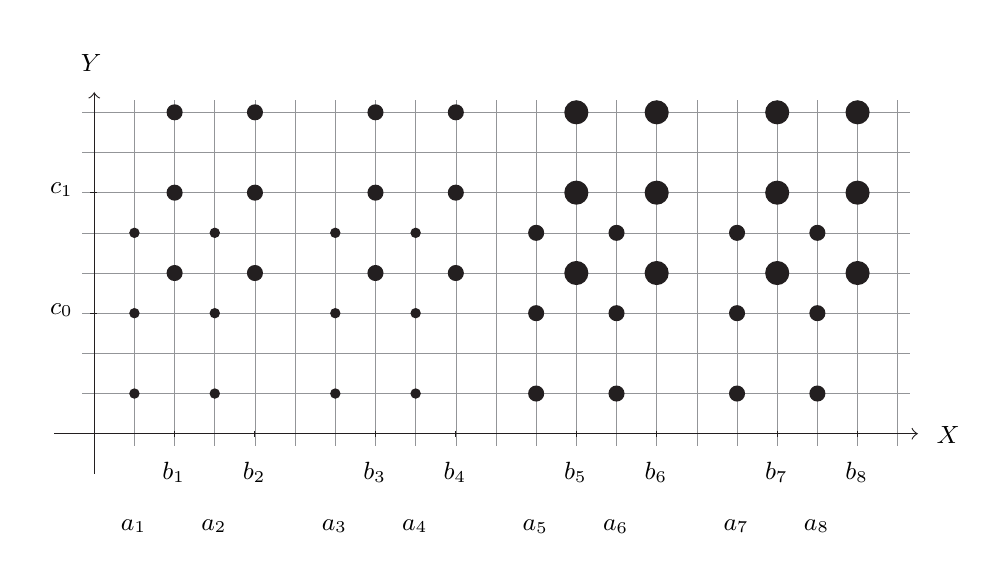
\begin{tikzpicture}[x=0.045cm,y=-0.045cm]
\useasboundingbox (0,0) rectangle (267,150);
\path[fill=none,draw=chfourfig3c0,line width=0.1992pt,draw opacity=1.0] (15.3874,114.5960) --(248.9616,114.5960) (15.3874,103.2575) --(248.9616,103.2575) (15.3874,91.9189) --(248.9616,91.9189) (15.3874,80.5804) --(248.9616,80.5804) (15.3874,69.2418) --(248.9616,69.2418) (15.3874,57.9033) --(248.9616,57.9033) (15.3874,46.5647) --(248.9616,46.5647) (15.3874,35.2262) --(248.9616,35.2262) (15.3874,23.8876) --(248.9616,23.8876) (18.7890,117.9976) --(18.7890,20.4860) (30.1275,117.9976) --(30.1275,20.4860) (41.4661,117.9976) --(41.4661,20.4860) (52.8046,117.9976) --(52.8046,20.4860) (64.1432,117.9976) --(64.1432,20.4860) (75.4818,117.9976) --(75.4818,20.4860) (86.8203,117.9976) --(86.8203,20.4860) (98.1588,117.9976) --(98.1588,20.4860) (109.4974,117.9976) --(109.4974,20.4860) (120.8359,117.9976) --(120.8359,20.4860) (132.1745,117.9976) --(132.1745,20.4860) (143.5130,117.9976) --(143.5130,20.4860) (154.8516,117.9976) --(154.8516,20.4860) (166.1901,117.9976) --(166.1901,20.4860) (177.5287,117.9976) --(177.5287,20.4860) (188.8672,117.9976) --(188.8672,20.4860) (200.2058,117.9976) --(200.2058,20.4860) (211.5443,117.9976) --(211.5443,20.4860) (222.8829,117.9976) --(222.8829,20.4860) (234.2215,117.9976) --(234.2215,20.4860) (245.5600,117.9976) --(245.5600,20.4860);
\path[fill=none,draw=chfourfig3c1,line width=0.3985pt,draw opacity=1.0] (7.4505,114.5960) --(250.7710,114.5960);
\path[fill=none,draw=chfourfig3c1,line width=0.3188pt,draw opacity=1.0] (249.5755,113.0020) .. controls (249.6751,113.5997) and (250.7710,114.4964) ..(251.0699,114.5960) .. controls (250.7710,114.6956) and (249.6751,115.5923) ..(249.5755,116.1900);
\path[fill=none,draw=chfourfig3c1,line width=0.3985pt,draw opacity=1.0] (18.7890,125.9346) --(18.7890,18.6766);
\path[fill=none,draw=chfourfig3c1,line width=0.3188pt,draw opacity=1.0] (17.1950,19.8721) .. controls (17.7927,19.7725) and (18.6894,18.6766) ..(18.7890,18.3778) .. controls (18.8886,18.6766) and (19.7853,19.7725) ..(20.3830,19.8721);
\path[fill=chfourfig3c1,fill opacity=1.0,draw=none] (31.6016,103.2575) .. controls (31.6016,102.4434) and (30.9416,101.7834) ..(30.1275,101.7834) .. controls (29.3134,101.7834) and (28.6535,102.4434) ..(28.6535,103.2575) .. controls (28.6535,104.0716) and (29.3134,104.7315) ..(30.1275,104.7315) .. controls (30.9416,104.7315) and (31.6016,104.0716) ..(31.6016,103.2575);
\path[fill=chfourfig3c1,fill opacity=1.0,draw=none] (54.2787,103.2575) .. controls (54.2787,102.4434) and (53.6187,101.7834) ..(52.8046,101.7834) .. controls (51.9905,101.7834) and (51.3306,102.4434) ..(51.3306,103.2575) .. controls (51.3306,104.0716) and (51.9905,104.7315) ..(52.8046,104.7315) .. controls (53.6187,104.7315) and (54.2787,104.0716) ..(54.2787,103.2575);
\path[fill=chfourfig3c1,fill opacity=1.0,draw=none] (43.7337,69.2418) .. controls (43.7337,67.9894) and (42.7185,66.9742) ..(41.4661,66.9742) .. controls (40.2137,66.9742) and (39.1984,67.9894) ..(39.1984,69.2418) .. controls (39.1984,70.4942) and (40.2137,71.5095) ..(41.4661,71.5095) .. controls (42.7185,71.5095) and (43.7337,70.4942) ..(43.7337,69.2418);
\path[fill=chfourfig3c1,fill opacity=1.0,draw=none] (66.4108,69.2418) .. controls (66.4108,67.9894) and (65.3956,66.9742) ..(64.1432,66.9742) .. controls (62.8908,66.9742) and (61.8755,67.9894) ..(61.8755,69.2418) .. controls (61.8755,70.4942) and (62.8908,71.5095) ..(64.1432,71.5095) .. controls (65.3956,71.5095) and (66.4108,70.4942) ..(66.4108,69.2418);
\path[fill=chfourfig3c1,fill opacity=1.0,draw=none] (31.6016,80.5804) .. controls (31.6016,79.7663) and (30.9416,79.1063) ..(30.1275,79.1063) .. controls (29.3134,79.1063) and (28.6535,79.7663) ..(28.6535,80.5804) .. controls (28.6535,81.3945) and (29.3134,82.0544) ..(30.1275,82.0544) .. controls (30.9416,82.0544) and (31.6016,81.3945) ..(31.6016,80.5804);
\path[fill=chfourfig3c1,fill opacity=1.0,draw=none] (54.2787,80.5804) .. controls (54.2787,79.7663) and (53.6187,79.1063) ..(52.8046,79.1063) .. controls (51.9905,79.1063) and (51.3306,79.7663) ..(51.3306,80.5804) .. controls (51.3306,81.3945) and (51.9905,82.0544) ..(52.8046,82.0544) .. controls (53.6187,82.0544) and (54.2787,81.3945) ..(54.2787,80.5804);
\path[fill=chfourfig3c1,fill opacity=1.0,draw=none] (43.7337,46.5647) .. controls (43.7337,45.3123) and (42.7185,44.2971) ..(41.4661,44.2971) .. controls (40.2137,44.2971) and (39.1984,45.3123) ..(39.1984,46.5647) .. controls (39.1984,47.8171) and (40.2137,48.8324) ..(41.4661,48.8324) .. controls (42.7185,48.8324) and (43.7337,47.8171) ..(43.7337,46.5647);
\path[fill=chfourfig3c1,fill opacity=1.0,draw=none] (66.4108,46.5647) .. controls (66.4108,45.3123) and (65.3956,44.2971) ..(64.1432,44.2971) .. controls (62.8908,44.2971) and (61.8755,45.3123) ..(61.8755,46.5647) .. controls (61.8755,47.8171) and (62.8908,48.8324) ..(64.1432,48.8324) .. controls (65.3956,48.8324) and (66.4108,47.8171) ..(66.4108,46.5647);
\path[fill=chfourfig3c1,fill opacity=1.0,draw=none] (31.6016,57.9033) .. controls (31.6016,57.0892) and (30.9416,56.4292) ..(30.1275,56.4292) .. controls (29.3134,56.4292) and (28.6535,57.0892) ..(28.6535,57.9033) .. controls (28.6535,58.7174) and (29.3134,59.3773) ..(30.1275,59.3773) .. controls (30.9416,59.3773) and (31.6016,58.7174) ..(31.6016,57.9033);
\path[fill=chfourfig3c1,fill opacity=1.0,draw=none] (54.2787,57.9033) .. controls (54.2787,57.0892) and (53.6187,56.4292) ..(52.8046,56.4292) .. controls (51.9905,56.4292) and (51.3306,57.0892) ..(51.3306,57.9033) .. controls (51.3306,58.7174) and (51.9905,59.3773) ..(52.8046,59.3773) .. controls (53.6187,59.3773) and (54.2787,58.7174) ..(54.2787,57.9033);
\path[fill=chfourfig3c1,fill opacity=1.0,draw=none] (43.7337,23.8876) .. controls (43.7337,22.6352) and (42.7185,21.6199) ..(41.4661,21.6199) .. controls (40.2137,21.6199) and (39.1984,22.6352) ..(39.1984,23.8876) .. controls (39.1984,25.1400) and (40.2137,26.1553) ..(41.4661,26.1553) .. controls (42.7185,26.1553) and (43.7337,25.1400) ..(43.7337,23.8876);
\path[fill=chfourfig3c1,fill opacity=1.0,draw=none] (66.4108,23.8876) .. controls (66.4108,22.6352) and (65.3956,21.6199) ..(64.1432,21.6199) .. controls (62.8908,21.6199) and (61.8755,22.6352) ..(61.8755,23.8876) .. controls (61.8755,25.1400) and (62.8908,26.1553) ..(64.1432,26.1553) .. controls (65.3956,26.1553) and (66.4108,25.1400) ..(66.4108,23.8876);
\path[fill=chfourfig3c1,fill opacity=1.0,draw=none] (88.2944,103.2575) .. controls (88.2944,102.4434) and (87.6344,101.7834) ..(86.8203,101.7834) .. controls (86.0062,101.7834) and (85.3463,102.4434) ..(85.3463,103.2575) .. controls (85.3463,104.0716) and (86.0062,104.7315) ..(86.8203,104.7315) .. controls (87.6344,104.7315) and (88.2944,104.0716) ..(88.2944,103.2575);
\path[fill=chfourfig3c1,fill opacity=1.0,draw=none] (110.9715,103.2575) .. controls (110.9715,102.4434) and (110.3115,101.7834) ..(109.4974,101.7834) .. controls (108.6833,101.7834) and (108.0233,102.4434) ..(108.0233,103.2575) .. controls (108.0233,104.0716) and (108.6833,104.7315) ..(109.4974,104.7315) .. controls (110.3115,104.7315) and (110.9715,104.0716) ..(110.9715,103.2575);
\path[fill=chfourfig3c1,fill opacity=1.0,draw=none] (100.4265,69.2418) .. controls (100.4265,67.9894) and (99.4112,66.9742) ..(98.1588,66.9742) .. controls (96.9064,66.9742) and (95.8912,67.9894) ..(95.8912,69.2418) .. controls (95.8912,70.4942) and (96.9064,71.5095) ..(98.1588,71.5095) .. controls (99.4112,71.5095) and (100.4265,70.4942) ..(100.4265,69.2418);
\path[fill=chfourfig3c1,fill opacity=1.0,draw=none] (123.1036,69.2418) .. controls (123.1036,67.9894) and (122.0883,66.9742) ..(120.8359,66.9742) .. controls (119.5835,66.9742) and (118.5683,67.9894) ..(118.5683,69.2418) .. controls (118.5683,70.4942) and (119.5835,71.5095) ..(120.8359,71.5095) .. controls (122.0883,71.5095) and (123.1036,70.4942) ..(123.1036,69.2418);
\path[fill=chfourfig3c1,fill opacity=1.0,draw=none] (88.2944,80.5804) .. controls (88.2944,79.7663) and (87.6344,79.1063) ..(86.8203,79.1063) .. controls (86.0062,79.1063) and (85.3463,79.7663) ..(85.3463,80.5804) .. controls (85.3463,81.3945) and (86.0062,82.0544) ..(86.8203,82.0544) .. controls (87.6344,82.0544) and (88.2944,81.3945) ..(88.2944,80.5804);
\path[fill=chfourfig3c1,fill opacity=1.0,draw=none] (110.9715,80.5804) .. controls (110.9715,79.7663) and (110.3115,79.1063) ..(109.4974,79.1063) .. controls (108.6833,79.1063) and (108.0233,79.7663) ..(108.0233,80.5804) .. controls (108.0233,81.3945) and (108.6833,82.0544) ..(109.4974,82.0544) .. controls (110.3115,82.0544) and (110.9715,81.3945) ..(110.9715,80.5804);
\path[fill=chfourfig3c1,fill opacity=1.0,draw=none] (100.4265,46.5647) .. controls (100.4265,45.3123) and (99.4112,44.2971) ..(98.1588,44.2971) .. controls (96.9064,44.2971) and (95.8912,45.3123) ..(95.8912,46.5647) .. controls (95.8912,47.8171) and (96.9064,48.8324) ..(98.1588,48.8324) .. controls (99.4112,48.8324) and (100.4265,47.8171) ..(100.4265,46.5647);
\path[fill=chfourfig3c1,fill opacity=1.0,draw=none] (123.1036,46.5647) .. controls (123.1036,45.3123) and (122.0883,44.2971) ..(120.8359,44.2971) .. controls (119.5835,44.2971) and (118.5683,45.3123) ..(118.5683,46.5647) .. controls (118.5683,47.8171) and (119.5835,48.8324) ..(120.8359,48.8324) .. controls (122.0883,48.8324) and (123.1036,47.8171) ..(123.1036,46.5647);
\path[fill=chfourfig3c1,fill opacity=1.0,draw=none] (88.2944,57.9033) .. controls (88.2944,57.0892) and (87.6344,56.4292) ..(86.8203,56.4292) .. controls (86.0062,56.4292) and (85.3463,57.0892) ..(85.3463,57.9033) .. controls (85.3463,58.7174) and (86.0062,59.3773) ..(86.8203,59.3773) .. controls (87.6344,59.3773) and (88.2944,58.7174) ..(88.2944,57.9033);
\path[fill=chfourfig3c1,fill opacity=1.0,draw=none] (110.9715,57.9033) .. controls (110.9715,57.0892) and (110.3115,56.4292) ..(109.4974,56.4292) .. controls (108.6833,56.4292) and (108.0233,57.0892) ..(108.0233,57.9033) .. controls (108.0233,58.7174) and (108.6833,59.3773) ..(109.4974,59.3773) .. controls (110.3115,59.3773) and (110.9715,58.7174) ..(110.9715,57.9033);
\path[fill=chfourfig3c1,fill opacity=1.0,draw=none] (100.4265,23.8876) .. controls (100.4265,22.6352) and (99.4112,21.6199) ..(98.1588,21.6199) .. controls (96.9064,21.6199) and (95.8912,22.6352) ..(95.8912,23.8876) .. controls (95.8912,25.1400) and (96.9064,26.1553) ..(98.1588,26.1553) .. controls (99.4112,26.1553) and (100.4265,25.1400) ..(100.4265,23.8876);
\path[fill=chfourfig3c1,fill opacity=1.0,draw=none] (123.1036,23.8876) .. controls (123.1036,22.6352) and (122.0883,21.6199) ..(120.8359,21.6199) .. controls (119.5835,21.6199) and (118.5683,22.6352) ..(118.5683,23.8876) .. controls (118.5683,25.1400) and (119.5835,26.1553) ..(120.8359,26.1553) .. controls (122.0883,26.1553) and (123.1036,25.1400) ..(123.1036,23.8876);
\path[fill=chfourfig3c1,fill opacity=1.0,draw=none] (145.7807,103.2575) .. controls (145.7807,102.0051) and (144.7654,100.9898) ..(143.5130,100.9898) .. controls (142.2607,100.9898) and (141.2454,102.0051) ..(141.2454,103.2575) .. controls (141.2454,104.5099) and (142.2607,105.5251) ..(143.5130,105.5251) .. controls (144.7654,105.5251) and (145.7807,104.5099) ..(145.7807,103.2575);
\path[fill=chfourfig3c1,fill opacity=1.0,draw=none] (168.4578,103.2575) .. controls (168.4578,102.0051) and (167.4425,100.9898) ..(166.1901,100.9898) .. controls (164.9377,100.9898) and (163.9225,102.0051) ..(163.9225,103.2575) .. controls (163.9225,104.5099) and (164.9377,105.5251) ..(166.1901,105.5251) .. controls (167.4425,105.5251) and (168.4578,104.5099) ..(168.4578,103.2575);
\path[fill=chfourfig3c1,fill opacity=1.0,draw=none] (158.2532,69.2418) .. controls (158.2532,67.3632) and (156.7303,65.8402) ..(154.8516,65.8402) .. controls (152.9729,65.8402) and (151.4500,67.3632) ..(151.4500,69.2418) .. controls (151.4500,71.1205) and (152.9729,72.6434) ..(154.8516,72.6434) .. controls (156.7303,72.6434) and (158.2532,71.1205) ..(158.2532,69.2418);
\path[fill=chfourfig3c1,fill opacity=1.0,draw=none] (180.9303,69.2418) .. controls (180.9303,67.3632) and (179.4073,65.8402) ..(177.5287,65.8402) .. controls (175.6500,65.8402) and (174.1271,67.3632) ..(174.1271,69.2418) .. controls (174.1271,71.1205) and (175.6500,72.6434) ..(177.5287,72.6434) .. controls (179.4073,72.6434) and (180.9303,71.1205) ..(180.9303,69.2418);
\path[fill=chfourfig3c1,fill opacity=1.0,draw=none] (145.7807,80.5804) .. controls (145.7807,79.3280) and (144.7654,78.3127) ..(143.5130,78.3127) .. controls (142.2607,78.3127) and (141.2454,79.3280) ..(141.2454,80.5804) .. controls (141.2454,81.8328) and (142.2607,82.8480) ..(143.5130,82.8480) .. controls (144.7654,82.8480) and (145.7807,81.8328) ..(145.7807,80.5804);
\path[fill=chfourfig3c1,fill opacity=1.0,draw=none] (168.4578,80.5804) .. controls (168.4578,79.3280) and (167.4425,78.3127) ..(166.1901,78.3127) .. controls (164.9377,78.3127) and (163.9225,79.3280) ..(163.9225,80.5804) .. controls (163.9225,81.8328) and (164.9377,82.8480) ..(166.1901,82.8480) .. controls (167.4425,82.8480) and (168.4578,81.8328) ..(168.4578,80.5804);
\path[fill=chfourfig3c1,fill opacity=1.0,draw=none] (158.2532,46.5647) .. controls (158.2532,44.6861) and (156.7303,43.1631) ..(154.8516,43.1631) .. controls (152.9729,43.1631) and (151.4500,44.6861) ..(151.4500,46.5647) .. controls (151.4500,48.4434) and (152.9729,49.9663) ..(154.8516,49.9663) .. controls (156.7303,49.9663) and (158.2532,48.4434) ..(158.2532,46.5647);
\path[fill=chfourfig3c1,fill opacity=1.0,draw=none] (180.9303,46.5647) .. controls (180.9303,44.6861) and (179.4073,43.1631) ..(177.5287,43.1631) .. controls (175.6500,43.1631) and (174.1271,44.6861) ..(174.1271,46.5647) .. controls (174.1271,48.4434) and (175.6500,49.9663) ..(177.5287,49.9663) .. controls (179.4073,49.9663) and (180.9303,48.4434) ..(180.9303,46.5647);
\path[fill=chfourfig3c1,fill opacity=1.0,draw=none] (145.7807,57.9033) .. controls (145.7807,56.6509) and (144.7654,55.6356) ..(143.5130,55.6356) .. controls (142.2607,55.6356) and (141.2454,56.6509) ..(141.2454,57.9033) .. controls (141.2454,59.1557) and (142.2607,60.1709) ..(143.5130,60.1709) .. controls (144.7654,60.1709) and (145.7807,59.1557) ..(145.7807,57.9033);
\path[fill=chfourfig3c1,fill opacity=1.0,draw=none] (168.4578,57.9033) .. controls (168.4578,56.6509) and (167.4425,55.6356) ..(166.1901,55.6356) .. controls (164.9377,55.6356) and (163.9225,56.6509) ..(163.9225,57.9033) .. controls (163.9225,59.1557) and (164.9377,60.1709) ..(166.1901,60.1709) .. controls (167.4425,60.1709) and (168.4578,59.1557) ..(168.4578,57.9033);
\path[fill=chfourfig3c1,fill opacity=1.0,draw=none] (158.2532,23.8876) .. controls (158.2532,22.0090) and (156.7303,20.4860) ..(154.8516,20.4860) .. controls (152.9729,20.4860) and (151.4500,22.0090) ..(151.4500,23.8876) .. controls (151.4500,25.7663) and (152.9729,27.2892) ..(154.8516,27.2892) .. controls (156.7303,27.2892) and (158.2532,25.7663) ..(158.2532,23.8876);
\path[fill=chfourfig3c1,fill opacity=1.0,draw=none] (180.9303,23.8876) .. controls (180.9303,22.0090) and (179.4073,20.4860) ..(177.5287,20.4860) .. controls (175.6500,20.4860) and (174.1271,22.0090) ..(174.1271,23.8876) .. controls (174.1271,25.7663) and (175.6500,27.2892) ..(177.5287,27.2892) .. controls (179.4073,27.2892) and (180.9303,25.7663) ..(180.9303,23.8876);
\path[fill=chfourfig3c1,fill opacity=1.0,draw=none] (202.4734,103.2575) .. controls (202.4734,102.0051) and (201.4582,100.9898) ..(200.2058,100.9898) .. controls (198.9534,100.9898) and (197.9381,102.0051) ..(197.9381,103.2575) .. controls (197.9381,104.5099) and (198.9534,105.5251) ..(200.2058,105.5251) .. controls (201.4582,105.5251) and (202.4734,104.5099) ..(202.4734,103.2575);
\path[fill=chfourfig3c1,fill opacity=1.0,draw=none] (225.1506,103.2575) .. controls (225.1506,102.0051) and (224.1353,100.9898) ..(222.8829,100.9898) .. controls (221.6305,100.9898) and (220.6152,102.0051) ..(220.6152,103.2575) .. controls (220.6152,104.5099) and (221.6305,105.5251) ..(222.8829,105.5251) .. controls (224.1353,105.5251) and (225.1506,104.5099) ..(225.1506,103.2575);
\path[fill=chfourfig3c1,fill opacity=1.0,draw=none] (214.9459,69.2418) .. controls (214.9459,67.3632) and (213.4230,65.8402) ..(211.5443,65.8402) .. controls (209.6657,65.8402) and (208.1428,67.3632) ..(208.1428,69.2418) .. controls (208.1428,71.1205) and (209.6657,72.6434) ..(211.5443,72.6434) .. controls (213.4230,72.6434) and (214.9459,71.1205) ..(214.9459,69.2418);
\path[fill=chfourfig3c1,fill opacity=1.0,draw=none] (237.6230,69.2418) .. controls (237.6230,67.3632) and (236.1001,65.8402) ..(234.2215,65.8402) .. controls (232.3428,65.8402) and (230.8199,67.3632) ..(230.8199,69.2418) .. controls (230.8199,71.1205) and (232.3428,72.6434) ..(234.2215,72.6434) .. controls (236.1001,72.6434) and (237.6230,71.1205) ..(237.6230,69.2418);
\path[fill=chfourfig3c1,fill opacity=1.0,draw=none] (202.4734,80.5804) .. controls (202.4734,79.3280) and (201.4582,78.3127) ..(200.2058,78.3127) .. controls (198.9534,78.3127) and (197.9381,79.3280) ..(197.9381,80.5804) .. controls (197.9381,81.8328) and (198.9534,82.8480) ..(200.2058,82.8480) .. controls (201.4582,82.8480) and (202.4734,81.8328) ..(202.4734,80.5804);
\path[fill=chfourfig3c1,fill opacity=1.0,draw=none] (225.1506,80.5804) .. controls (225.1506,79.3280) and (224.1353,78.3127) ..(222.8829,78.3127) .. controls (221.6305,78.3127) and (220.6152,79.3280) ..(220.6152,80.5804) .. controls (220.6152,81.8328) and (221.6305,82.8480) ..(222.8829,82.8480) .. controls (224.1353,82.8480) and (225.1506,81.8328) ..(225.1506,80.5804);
\path[fill=chfourfig3c1,fill opacity=1.0,draw=none] (214.9459,46.5647) .. controls (214.9459,44.6861) and (213.4230,43.1631) ..(211.5443,43.1631) .. controls (209.6657,43.1631) and (208.1428,44.6861) ..(208.1428,46.5647) .. controls (208.1428,48.4434) and (209.6657,49.9663) ..(211.5443,49.9663) .. controls (213.4230,49.9663) and (214.9459,48.4434) ..(214.9459,46.5647);
\path[fill=chfourfig3c1,fill opacity=1.0,draw=none] (237.6230,46.5647) .. controls (237.6230,44.6861) and (236.1001,43.1631) ..(234.2215,43.1631) .. controls (232.3428,43.1631) and (230.8199,44.6861) ..(230.8199,46.5647) .. controls (230.8199,48.4434) and (232.3428,49.9663) ..(234.2215,49.9663) .. controls (236.1001,49.9663) and (237.6230,48.4434) ..(237.6230,46.5647);
\path[fill=chfourfig3c1,fill opacity=1.0,draw=none] (202.4734,57.9033) .. controls (202.4734,56.6509) and (201.4582,55.6356) ..(200.2058,55.6356) .. controls (198.9534,55.6356) and (197.9381,56.6509) ..(197.9381,57.9033) .. controls (197.9381,59.1557) and (198.9534,60.1709) ..(200.2058,60.1709) .. controls (201.4582,60.1709) and (202.4734,59.1557) ..(202.4734,57.9033);
\path[fill=chfourfig3c1,fill opacity=1.0,draw=none] (225.1506,57.9033) .. controls (225.1506,56.6509) and (224.1353,55.6356) ..(222.8829,55.6356) .. controls (221.6305,55.6356) and (220.6152,56.6509) ..(220.6152,57.9033) .. controls (220.6152,59.1557) and (221.6305,60.1709) ..(222.8829,60.1709) .. controls (224.1353,60.1709) and (225.1506,59.1557) ..(225.1506,57.9033);
\path[fill=chfourfig3c1,fill opacity=1.0,draw=none] (214.9459,23.8876) .. controls (214.9459,22.0090) and (213.4230,20.4860) ..(211.5443,20.4860) .. controls (209.6657,20.4860) and (208.1428,22.0090) ..(208.1428,23.8876) .. controls (208.1428,25.7663) and (209.6657,27.2892) ..(211.5443,27.2892) .. controls (213.4230,27.2892) and (214.9459,25.7663) ..(214.9459,23.8876);
\path[fill=chfourfig3c1,fill opacity=1.0,draw=none] (237.6230,23.8876) .. controls (237.6230,22.0090) and (236.1001,20.4860) ..(234.2215,20.4860) .. controls (232.3428,20.4860) and (230.8199,22.0090) ..(230.8199,23.8876) .. controls (230.8199,25.7663) and (232.3428,27.2892) ..(234.2215,27.2892) .. controls (236.1001,27.2892) and (237.6230,25.7663) ..(237.6230,23.8876);
\path[fill=none,draw=chfourfig3c1,line width=0.3985pt,draw opacity=1.0] (41.4661,113.7990) --(41.4661,115.3930);
\path[fill=none,draw=chfourfig3c1,line width=0.3985pt,draw opacity=1.0] (64.1432,113.7990) --(64.1432,115.3930);
\path[fill=none,draw=chfourfig3c1,line width=0.3985pt,draw opacity=1.0] (98.1588,113.7990) --(98.1588,115.3930);
\path[fill=none,draw=chfourfig3c1,line width=0.3985pt,draw opacity=1.0] (120.8359,113.7990) --(120.8359,115.3930);
\path[fill=none,draw=chfourfig3c1,line width=0.3985pt,draw opacity=1.0] (154.8516,113.7990) --(154.8516,115.3930);
\path[fill=none,draw=chfourfig3c1,line width=0.3985pt,draw opacity=1.0] (177.5287,113.7990) --(177.5287,115.3930);
\path[fill=none,draw=chfourfig3c1,line width=0.3985pt,draw opacity=1.0] (211.5443,113.7990) --(211.5443,115.3930);
\path[fill=none,draw=chfourfig3c1,line width=0.3985pt,draw opacity=1.0] (234.2215,113.7990) --(234.2215,115.3930);
\path[fill=none,draw=chfourfig3c1,line width=0.3985pt,draw opacity=1.0] (17.5935,80.5804) --(19.5860,80.5804);
\path[fill=none,draw=chfourfig3c1,line width=0.3985pt,draw opacity=1.0] (17.5935,46.5647) --(19.5860,46.5647);
\node[font=\small,inner sep=0pt,rotate=0] (ch04f3t0) at (259.7976,115.0809) {$X$};
\node[font=\small,inner sep=0pt,rotate=0] (ch04f3t1) at (17.9076,9.9439) {$Y$};
\node[font=\small,inner sep=0pt,rotate=0] (ch04f3t2) at (29.8786,140.7084) {$a_1$};
\node[font=\small,inner sep=0pt,rotate=0] (ch04f3t3) at (52.5556,140.7084) {$a_2$};
\node[font=\small,inner sep=0pt,rotate=0] (ch04f3t4) at (86.5706,140.7084) {$a_3$};
\node[font=\small,inner sep=0pt,rotate=0] (ch04f3t5) at (109.2476,140.7084) {$a_4$};
\node[font=\small,inner sep=0pt,rotate=0] (ch04f3t6) at (143.2626,140.7599) {$a_5$};
\node[font=\small,inner sep=0pt,rotate=0] (ch04f3t7) at (165.9396,140.7599) {$a_6$};
\node[font=\small,inner sep=0pt,rotate=0] (ch04f3t8) at (199.9546,140.7084) {$a_7$};
\node[font=\small,inner sep=0pt,rotate=0] (ch04f3t9) at (222.6316,140.7084) {$a_8$};
\node[font=\small,inner sep=0pt,rotate=0] (ch04f3t10) at (41.2171,125.5584) {$b_1$};
\node[font=\small,inner sep=0pt,rotate=0] (ch04f3t11) at (63.8941,125.5584) {$b_2$};
\node[font=\small,inner sep=0pt,rotate=0] (ch04f3t12) at (97.9091,125.5584) {$b_3$};
\node[font=\small,inner sep=0pt,rotate=0] (ch04f3t13) at (120.5861,125.5584) {$b_4$};
\node[font=\small,inner sep=0pt,rotate=0] (ch04f3t14) at (154.6011,125.6099) {$b_5$};
\node[font=\small,inner sep=0pt,rotate=0] (ch04f3t15) at (177.2781,125.6099) {$b_6$};
\node[font=\small,inner sep=0pt,rotate=0] (ch04f3t16) at (211.2931,125.5584) {$b_7$};
\node[font=\small,inner sep=0pt,rotate=0] (ch04f3t17) at (233.9701,125.5584) {$b_8$};
\node[font=\small,inner sep=0pt,rotate=0] (ch04f3t18) at (9.5056,79.7139) {$c_0$};
\node[font=\small,inner sep=0pt,rotate=0] (ch04f3t19) at (9.5056,45.7554) {$c_1$};
\end{tikzpicture}
\caption{只有经过精心选择的参数，才容许两个方向上的加性噪声模型，见定理4.6。圆点半径对应概率值。定理中的集合为 $C_0=\{a_1,a_2,\ldots,a_8\}$ 和 $C_1=\{b_1,b_2,\ldots,b_8\}$；函数 $f$ 在 $C_0,C_1$ 上分别取值 $c_0,c_1$。}
\label{fig:ch04-3}
\end{figure}
